\subsection{Open Street Map}

text

\cite{osm}

\subsection{A Close Look at an Open Street Map Case Study}

\begin{figure}
\centering
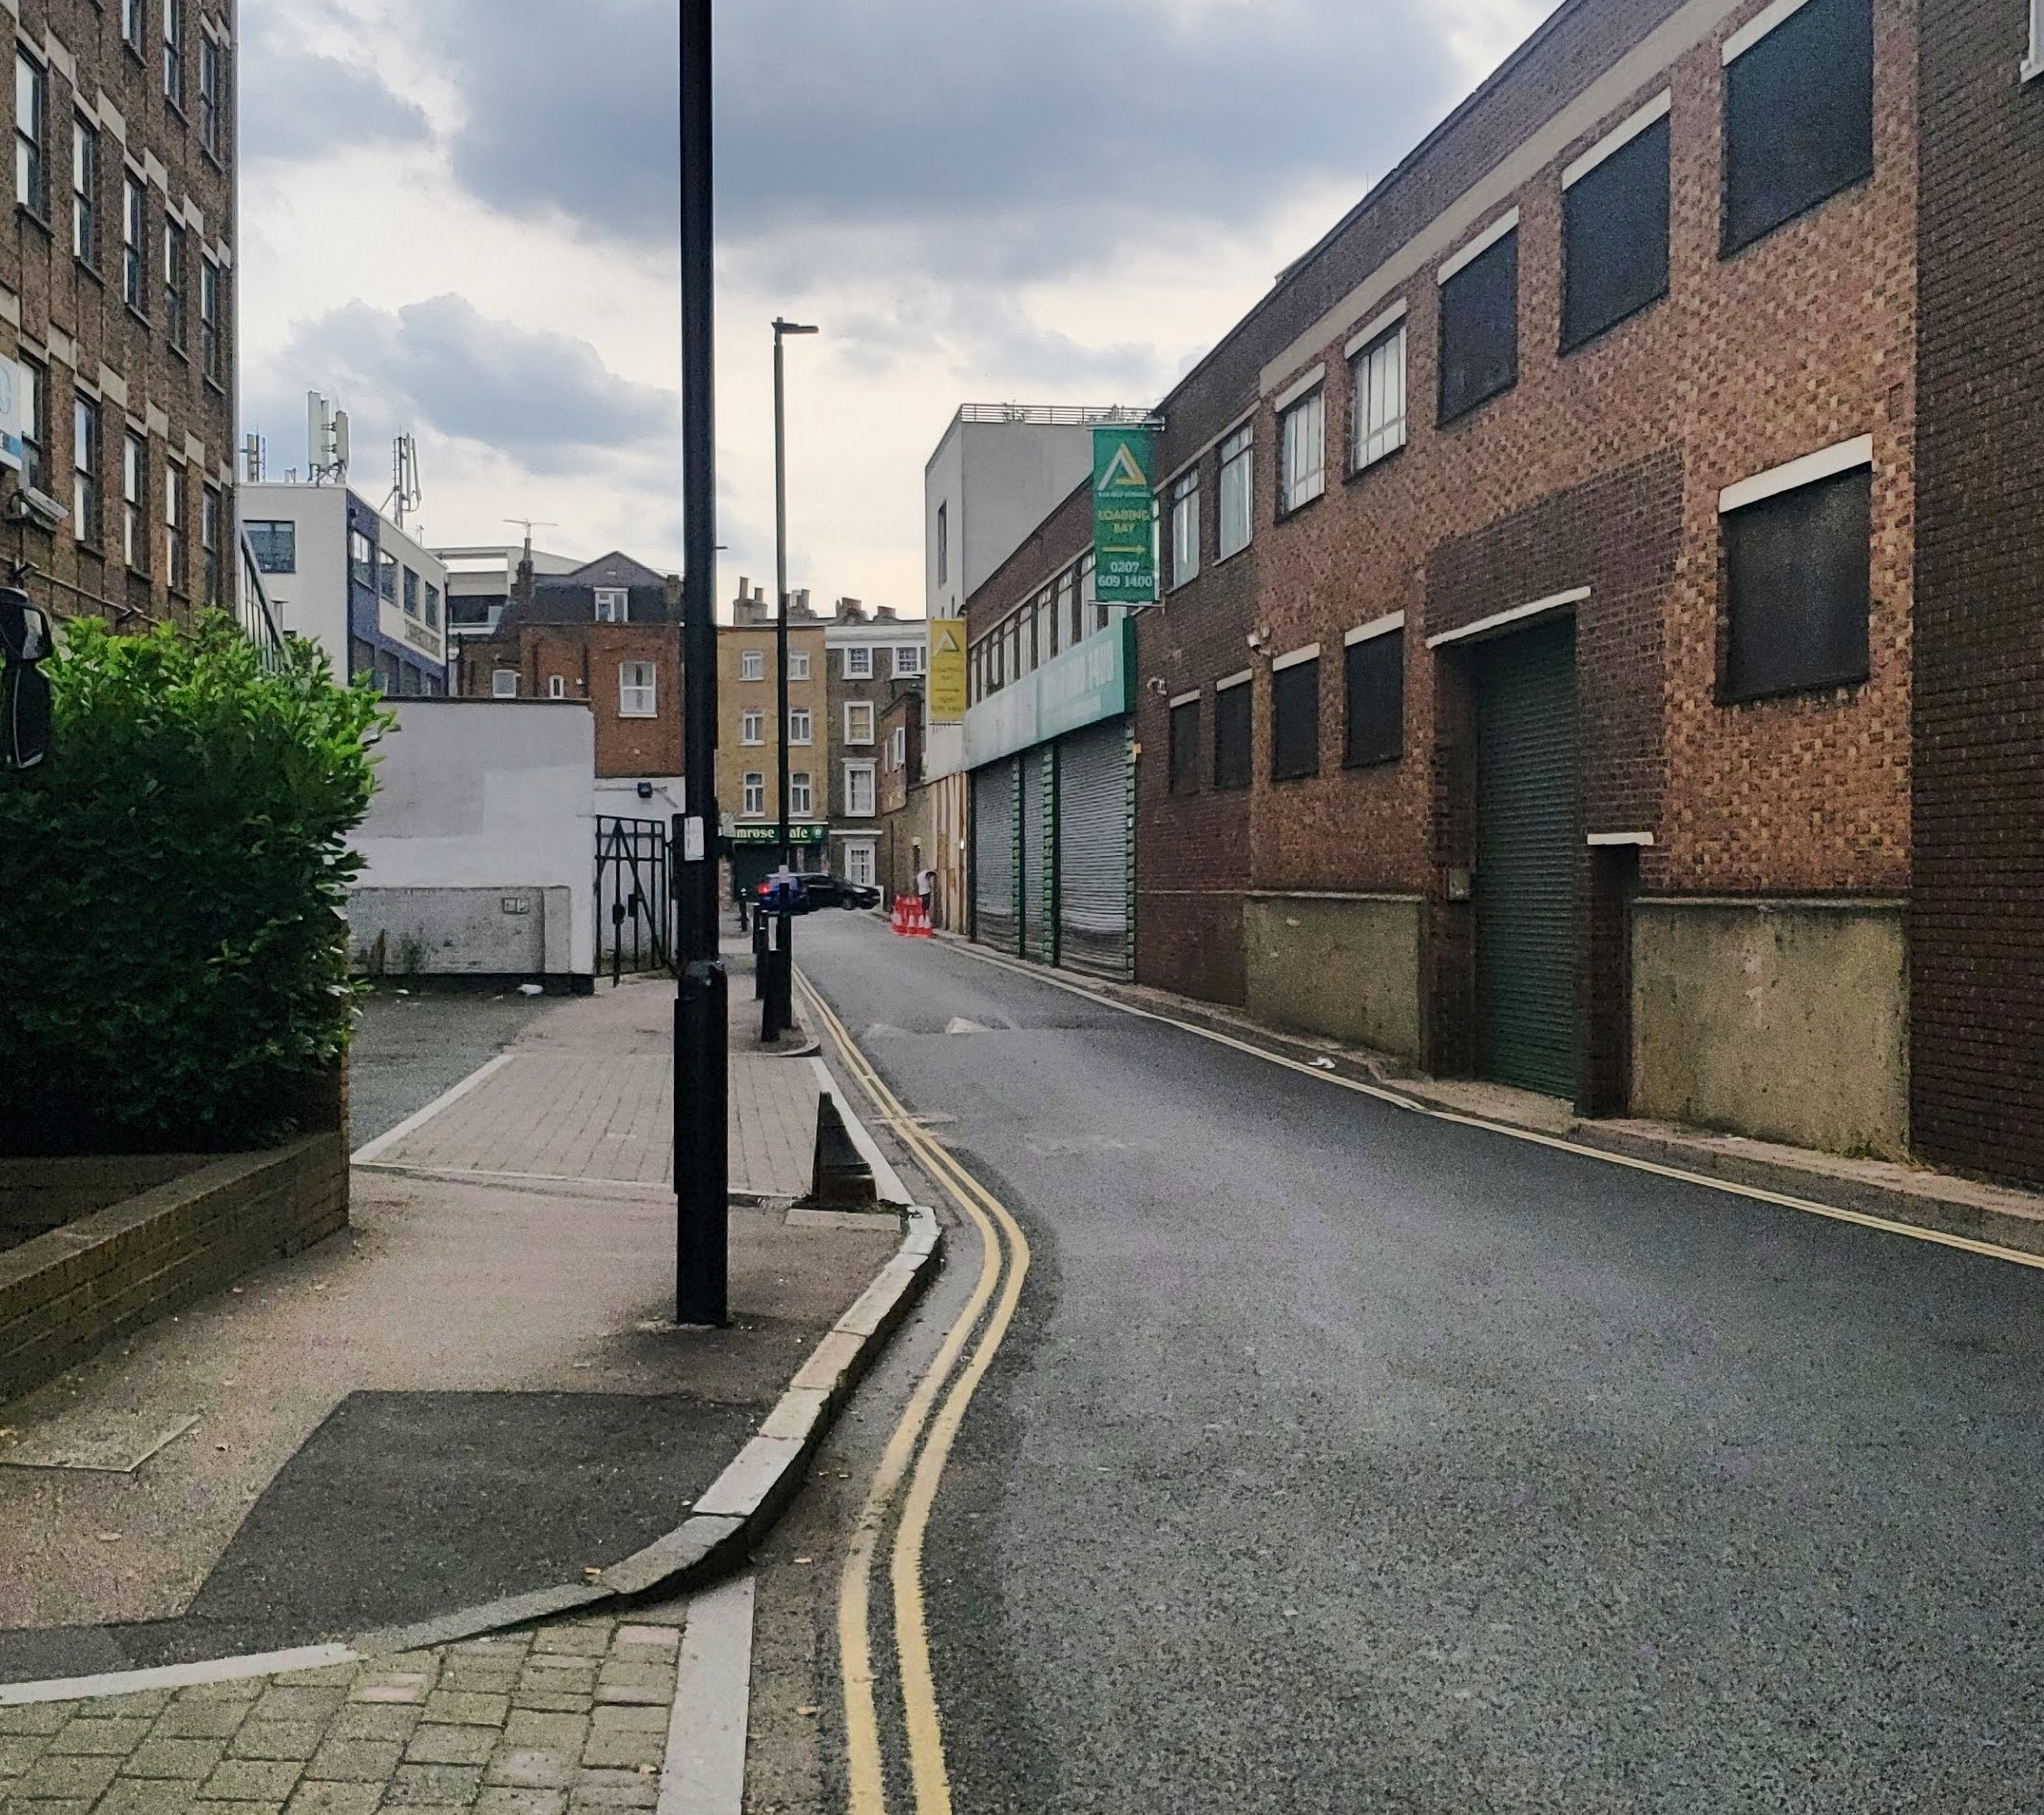
\includegraphics[width=0.6\textwidth]{brandon_rd_cropped}
\caption{image of quietway}
\end{figure}

\begin{figure}
\centering
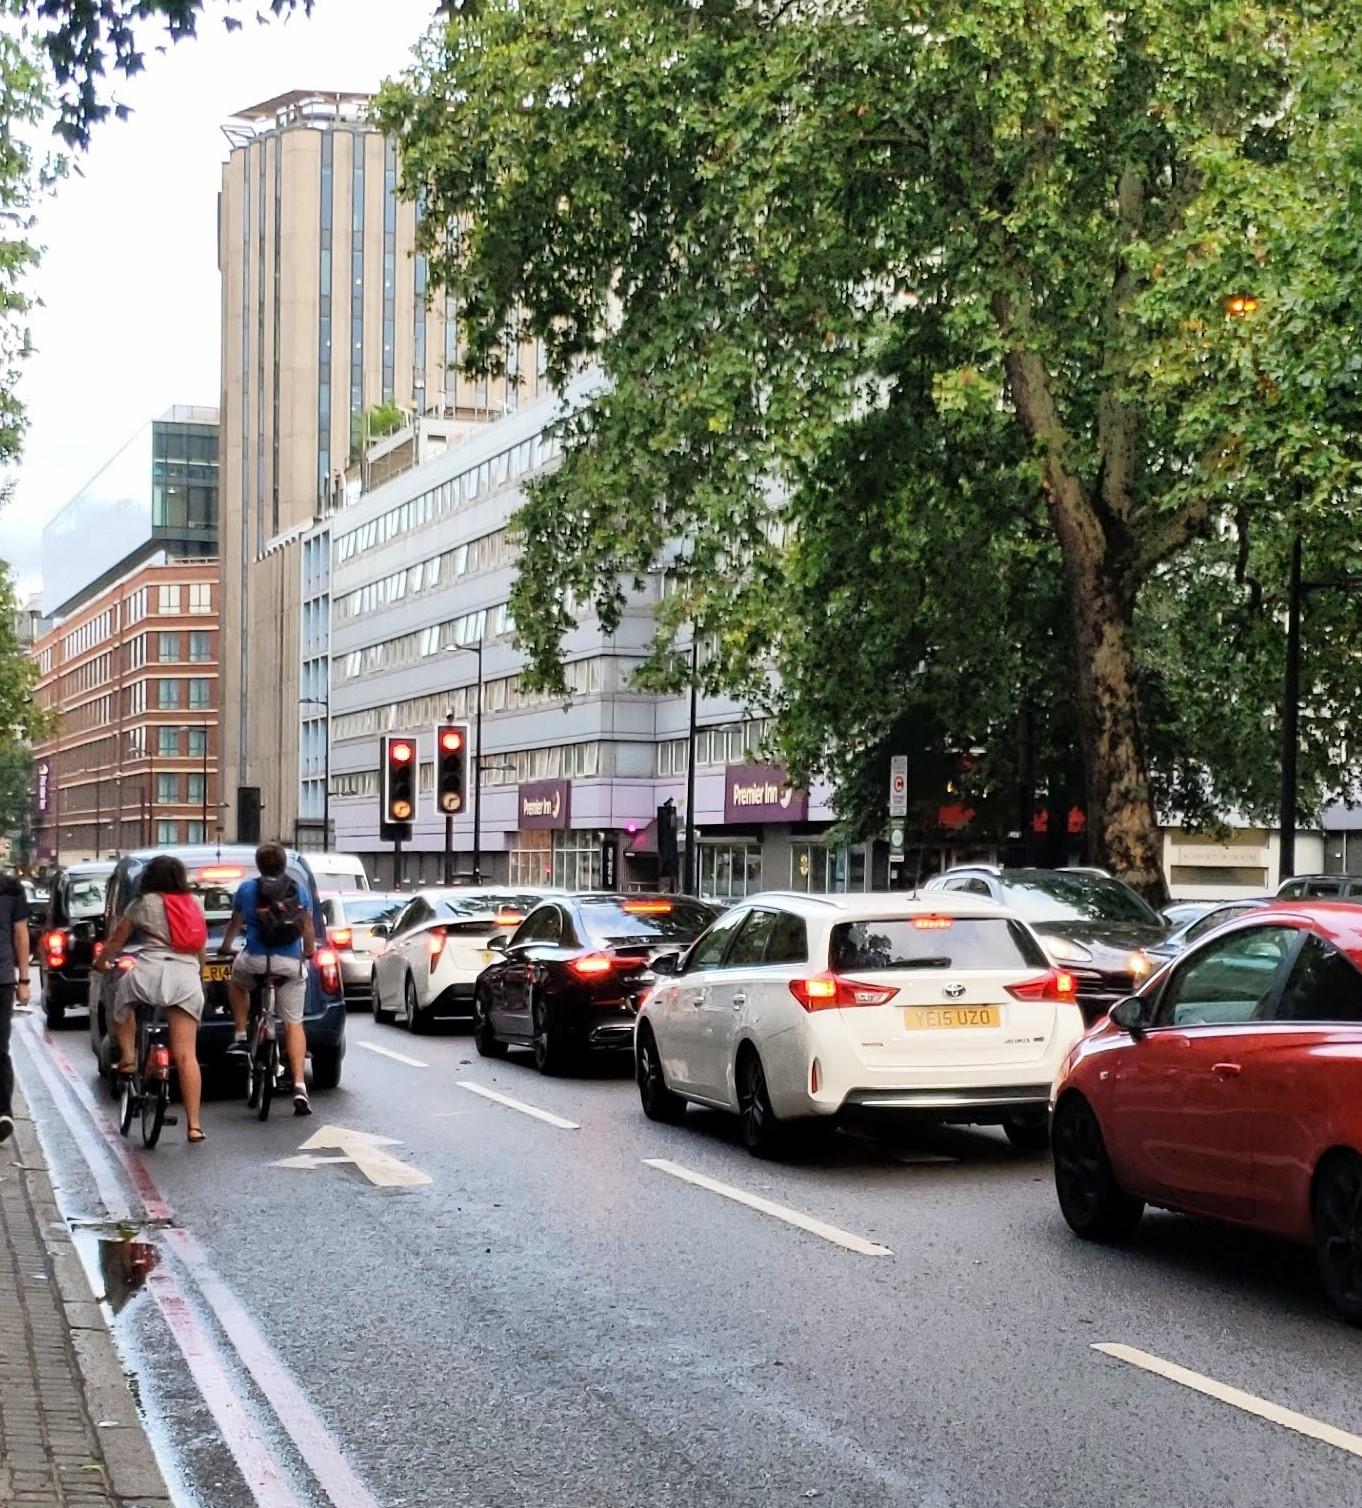
\includegraphics[width=0.6\textwidth]{euston_rd_cropped}
\caption{An image of Euston Road}
\label{fig:euston}
\end{figure}

\subsection{Transport for London Cycling Infrastructure Database}

\cite{tflcid}

osm effort to integrate
%https://wiki.openstreetmap.org/wiki/TfL_Cycling_Infrastructure_Database

\subsection{QUANT}

The QUANT dataset of public transport travel times was .

CITE

The of XXXX million pairs, XXXXX had not public transport link. To clean this data, the set is cut down to match the scope of the the investigation. Where there is no link between an origin destination pair, a link is constructed by combining the walking time from the origin to the node of highest degree in another LSOA where public transport is available to the destination LSOA. 

The walking speed used will be taken from google and the distance is the straightline distance between two points. This is less accurate than actually finding the walking route between the two points but this level of detail was not computationally feasible. 

\subsection{2011 Census Journey to work data}

The 2011 census asked each household where they lived, where they worked and how they traveled to work the preceding week. Thus data for origin and destination by mode of transport was available. This data will be used to help define the optimal scope. 

\cite{jtw}

\subsection{LSOA boundaries and data}
	
test citation for \cite{lsoageoms}. Did it work?
	
\subsection{Road KSI data}
	
	
	works but the cictation isn't formatted correctly
	\cite{cyclistksi}
	
\subsection{Data import, storage, cleaning, and joining}

cite postgres
cite postgis
cited beaver
cite python
cite pandas
cite json
cite sqlachemy

text